\documentclass[a4paper,12pt, english]{article}
\usepackage[T1]{fontenc}
\usepackage[utf8]{inputenc}
\usepackage{graphicx}
\usepackage{babel}
\usepackage{amsmath}
\usepackage{ulem}
\usepackage{a4wide}
\usepackage{graphicx}
\usepackage{listings}
\usepackage{tabularx}
\usepackage{tabulary}

\title{FYS3150 - Prosjekt 2}
\author{John-Anders Stende}

\begin{document}

\section*{Introduction}

The aim of this project is to develop a code for simulating the solar system using the Runge-Kutta-4 (RK4) algorithm.

I will do this gradually by first setting up the coupled differential equations for the two-body problem Sun-Earth. These equations then need to be discretized and implemented in an RK4 solver. To test the RK4 algorithm I will compare the results to known closed-form solutions to this problem for different time steps $h$ 

Adding Jupiter results in a three-body problem. The differential equations for Earth then needs to be rewritten to account for the gravity of one more object. The aim of this set-up is to investigate how Jupiter alters Earth's orbit around the Sun. I will also discuss the stability of the RK4 solver when Jupiter's mass is increased for different $h$.

Finally, I will add the seven other planets to simulate the solar system and compare the results with the earlier problems. 

\section*{Runge-Kutta-4 algorithm}

RK4 is an iterative algorithm that approximates solutions to ordinary differential equations. It is based on Taylor expansion like Euler's method, but uses intermediate steps to find the slope when computing the next function value. These intermediate values are however computed with Euler's method. Consider the following definitions:
\[
\frac{dx}{dt}=f(t,x), \ x(t)=\int f(t,x)dt
\]
and discretized
\[
x_{i+1} = x_i + \int_{t_i}^{t_{i+1}}f(t,x)dt
\]
The latter equation is a discretized version of the Taylor expansion
\[
x(t+h) = x(t) + hf(t,x)
\]
If we simply set $f(t,x) = dx/dt$ we have Euler's method. RK4 however, computes the integral of $f(t,x)$ using Simpson's method:
\[
\int_{t_i}^{t_{i+1}}f(t,x)dt = x_i + \frac{h}{6} \lbrack f(t_i,x_i) + 2f(t_i+h/2,x_{i+1/2}) +
2f(t_i+h/2,x_{i+1/2}) + f(t_i+h,x_{i+1}) \rbrack
\]
\[
= x_i + \frac{h}{6} (k1 + 2k2 + 2k3 + k4)
\]
thus RK4 computes four different slopes $k_i$ and uses a weighted average of these to compute $x_{i+1}$. RK4 can be viewed as a predict-and-correct algorithm. We first compute a slope $k_1$ and use this to predict $x_{i+1/2}$ with Euler's method. This value is used to compute a new slope $k_2$, and then we use this new slope to correct $x_{i+1/2}$ with Euler's method, and so on. The idea is to compute the slope at different places in the interval $\lbrack t_i,t_{i+1} \rbrack$ to obtain a final slope that fits the function $x(t)$ we want to find better.

\section*{Two-body problem Sun-Earth}

The only force in this problem is gravity, given by Newton's law of gravitation
\[
F=\frac{GM_{\mathrm{Sun}}M_{\mathrm{Earth}}}{r^2},
\]
where $M_{\mathrm{sun}}$ is the mass of the Sun and $M_{\mathrm{Earth}}$ is the mass of Earth. $G$ is the gravitational constant and $r$ is the distance between Earth and the Sun.

I will account for both the Sun and Earth's motion while placing the Sun in the center-of-mass position, the origin. This is almost equivalent with neglecting the Sun's motion because $M_{\mathrm{Sun}} >> M_{\mathrm{Earth}}$. To keep the center-of-mass fixed, I set the Sun's initial velocity so that the total linear momentum of the two-body system is zero.

I assume that the orbit of Earth around the Sun is co-planar, and I take this to be the $xy$-plane. Using Newton's second law of motion we get the following equations for Earth:
\[
\frac{d^2x}{dt^2}=\frac{F_x}{M_{\mathrm{Earth}}},
\]
and 
\[
\frac{d^2y}{dt^2}=\frac{F_y}{M_{\mathrm{Earth}}},
\]
where $F_x$ and $F_y$ are the $x$ and $y$ components of the gravitational force. The equations for the Sun can be obtained by replacing $M_{\mathrm{Earth}}$ with $M_{\mathrm{Sun}}$ in the following. 

The next step is to rewrite these second-order differential equations as a set of coupled first order differential equations in the following way:
\[
\frac{dx}{dt}=v_x, \ \frac{d^2x}{dt^2}=\frac{dv_x}{dt}=\frac{F_x}{M_{\mathrm{Earth}}},
\]
and
\[
\frac{dy}{dt}=v_y, \ \frac{d^2y}{dt^2}=\frac{dv_y}{dt}=\frac{F_y}{M_{\mathrm{Earth}}},
\]
where component-wise F is obtained like this:
\[
F_x = -\frac{GM_{Sun}M_{Earth}cos\theta}{r^2} = -\frac{GM_{Sun}M_{Earth}rcos\theta}{r^3} = 
-\frac{GM_{Sun}M_{Earth}x}{r^3}
\]
where $r=\sqrt{x^2+y^2}$. The equation for $F_y$ is obtained by replacing $x$ with $y$. The negative sign ensures that the $F$ from the Sun on Earth acts in the negative $x$-direction when $x_{Earth}$ is positive and vice versa.

Standard units become very impractical when simulating the solar system because the model we use span many years and large distances. I will therefore use the astronomical unit 
($1 AU = 1.5x10^{11} m$) instead of meters and years ($1 yr = 3.2x10^7 s$) instead of seconds.
The unit of $G$ can be obtained by using the fact that Earth's orbit around the Sun is almost circular, which means that the gravitational force $F$ must obey the centripetal force relation
\[
F = \frac{M_{\mathrm{Earth}}v^2}{r}=\frac{GM_{Sun}M_{\mathrm{Earth}}}{r^2},
\]
where $v$ is the velocity of Earth. The latter equation leads to
\[
v^2r=GM_{Sun}=4\pi^2\mathrm{AU}^3/\mathrm{yr}^2.
\]
If we in addition use Solar mass as mass unit we have $M_{Sun} = 1$ and 
$G = 4\pi^2$ with our new units. 

To implement the equations in a program, I need to discretize the system. Defining $t_i = t_0 + ih$ for $i = 0, 1, \dots , N-1$ where $N$ is the number of grid points and 
$h = \frac{t_{N-1} - t_0}{N}$ is the time step. Thus $x(t) \rightarrow x(t_i)$ and same for the velocities. The discretized equations (for $x$) that must be computed for each time step for Earth then becomes
\[
x_{i+1} = x_i + hv_i, \ v_{xi+1} = v_{xi} - \frac{GM_{Sun}x}{r^3}
\]
where $x = x_{Earth} - x_{Sun}$. 

\subsection*{Implementation}
My project consists of the three files $main.cpp$, $planet.cpp$ and $constants.cpp$. The first one is the main program, where I initialize the problem and make a $Planet$ class object for each body I'm working with. $planet.cpp$ contains the $Planet$ class, while $constants.cpp$ contains the global constants $\pi$, $G$ and $M_{Sun}$. $main.cpp$ is also where I've implemented a vectorized version of RK4 and the function $f$ that computes and returns the derivative of the system state vector $A$ (a vector containing the positions and velocities of the Sun and Earth). See the program files for further details.

\subsection*{Results}
The time development of the Sun-Earth system depends on the initial conditions of both objects. I discussed these for the Sun above. The function $lin_mom$ computes the linear momentum of Earth and $v_{y0}$ for the Sun is set on the basis of that value. I set $x_0 = 1 AU$ and 
$v_{y0} = 2\pi AU/yr$ for Earth to make sure that it completes one full round around the Sun in one year so that it's orbit becomes circular. The result for $t_{max} = 50$ and $N = 10000$ is shown in figure 1.

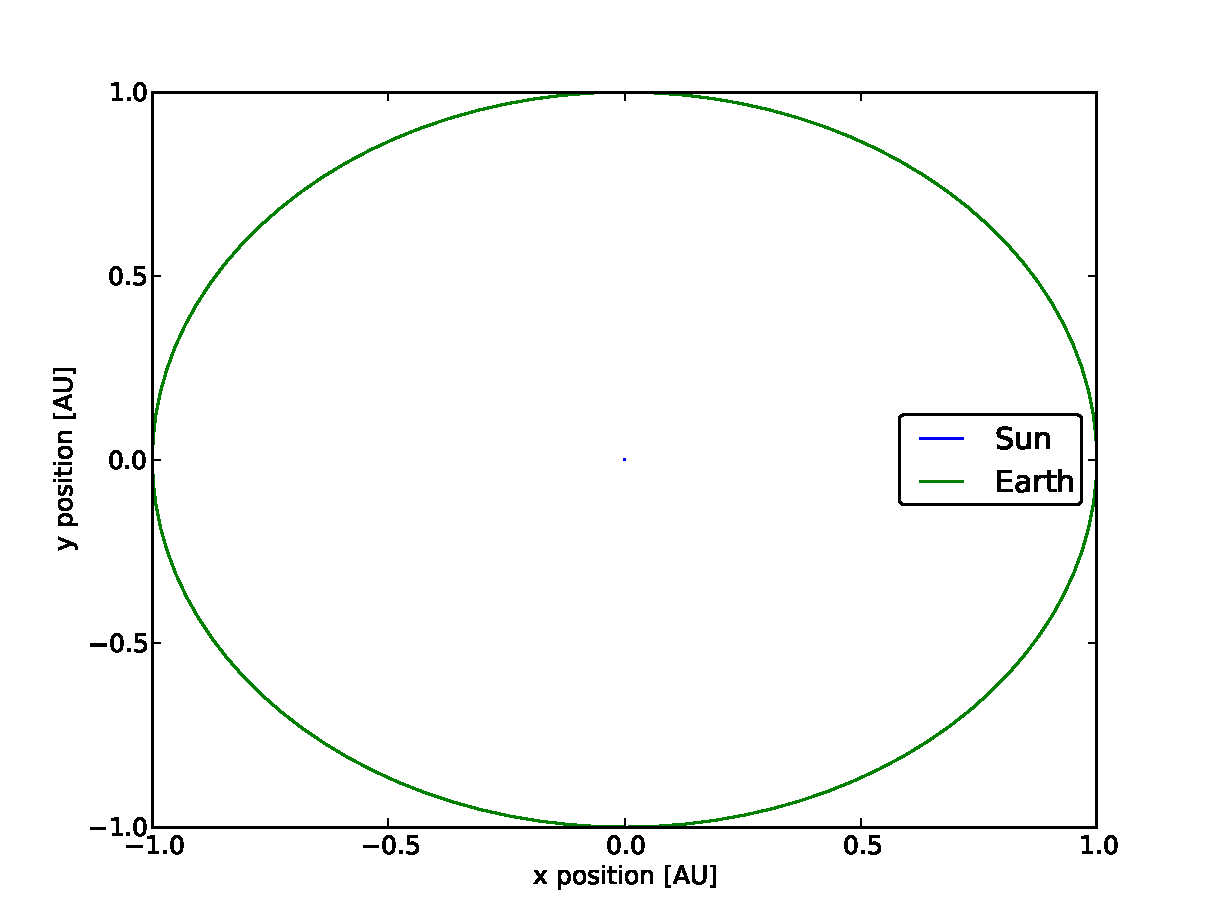
\includegraphics[scale = 0.5]{Fig1.pdf}













\end{document}
